\documentclass[10pt,a4paper]{article}
\usepackage[utf8]{inputenc}
\usepackage[spanish,english]{babel}
\usepackage{amsmath, amsfonts, amssymb}
\usepackage[backend=biber]{biblatex}
\bibliography{biblio.bib}
\usepackage[hidelinks]{hyperref}
\usepackage{csquotes}
\usepackage{graphicx}

\usepackage{color}
\usepackage{listings}

\definecolor{mygreen}{rgb}{0,0.6,0}
\definecolor{mygray}{rgb}{0.5,0.5,0.5}
\definecolor{mymauve}{rgb}{0.58,0,0.82}

\lstset{
  language=java,                   % sets language
  backgroundcolor=\color{white},   % choose the background color
  basicstyle=\footnotesize,        % size of fonts used for the code
  breaklines=true,                 % automatic line breaking only at whitespace
  captionpos=b,                    % sets the caption-position to bottom
  commentstyle=\color{mygreen},    % comment style
  escapeinside={\%*}{*)},          % if you want to add LaTeX within your code
  keywordstyle=\color{blue},       % keyword style
  stringstyle=\color{mymauve},     % string literal style
}

\author{Carlos Federico Gaona}
\title{Minería de Datos con WEKA \\ Notas de Curso}
\date{}

\begin{document}
\maketitle
\part{Conceptos}
\section{¿Qué es Minería de Datos?}
En \cite{larose2014discovering} tenemos, ``Minería de datos es el proceso de descubrir nuevas correlaciones y patrones, examinando cuidadosamente a través de grandes cantidades de datos almacenados en repositorios, utilizando tecnologías de reconocimiento de patrones como también técnicas estadísticas y matemáticas'', entre varias otras definiciones.

Sin embargo, esta actividad es un paso más dentro del proceso ``Descubrimiento de Conocimiento en Datos'' el cual engloba las actividades desde la obtención de los datos, su limpieza, la construcción de los modelos y su presentación final. En la actualidad el estándar CRISP-DM (Cross-Industry Standard Process for Data Mining) es el más utilizado \cite{oct2014poll} y detalla los siguientes pasos \cite{larose2014discovering}:
\begin{description}
\item[Business Understanding Phase] También llamado ``Research Understanding Phase''. Enuncia los objetivos claramente en términos del negocio/investigación. Traduce estos objetivos en términos de Minería de Datos.
\item[Data Undestanding Phase] Colecta los datos. Se familiariza con los datos utilizando Exploratory Data Analysis. Evalúa la calidad de los datos y selecciona los subconjuntos de interés según el paso anterior.
\item[Data Preparation Phase] Prepara los datos para ser procesados por pasos siguientes, es el paso mas laborioso. Selecciona y, de ser necesario, transforma las variables (atributos) que se consideran apropiadas para el paso siguiente.
\item[Modeling Phase] Alimenta los modelos con los datos preparados y los calibra para óptimo rendimiento. De ser necesario, se puede volver a pasos anteriores a preparar datos para un modelo en particular.
\item[Evaluation Phase] Determina si los modelos finales satisfacen los objetivos del primer paso.
\item[Deployment Phase] Hacer uso de los modelos, la construcción no es suficiente. Puede ser desde un simple reporte realizado por un experto hasta la reestructuración de la empresa según las recomendaciones del modelo.
\end{description}

En \cite{larose2014discovering} se detallan 5 casos de estudio del CRISP-DM y en \cite{crispdmpdf} podemos encontrar una copia. Debido a que CRISP-DM fue publicado inicialmente en 1999 y no ha presentado revisiones significativas\footnote{La pagina oficial \textit{crisp-dm.org} no esta activa en la actualidad, mayo 2016.} IBM ha presentado una mejora sobre CRISP-DM, ``Analytics Solutions Unified Method'' o ``ASUM-DM''\cite{asumdmarticle}.

\section{Conjunto de Datos, Instancias y Atributos}
\subsection{Instancias y atributos}
Cada instancia es la mínima unidad con la que trabajan los modelos. Cada instancia posee una serie de atributos que son las mediciones respectivas y pueden ser \textbf{numéricos} o \textbf{nominales}. Los atributos numéricos están caracterizado por un dominio continuo, como por ejemplo $2.718281$ o $-50$, y los atributos nominales por un dominio discreto, como por ejemplo \textit{BAJO}, \textit{MEDIO}, \textit{ALTO}.

Una instancia es una fila de la figura \ref{Table1} y un atributo es un campo. Se puede dar el caso de que el valor de un atributo de una instancia en particular se haya perdido o haya podido ser obtenido, en ese caso se considera el valor especial \textbf{perdido} y no todos los modelos son capaces de procesar este valor.

\subsection{Conjunto de Datos}
Usualmente los modelos se alimentan de conjuntos de datos, en inglés \textit{dataset}, que son conjuntos\footnote{En el estricto sentido matemático no son conjuntos ya que nada impide que la misma muestra aparezca varias veces.} de instancias donde una de ellas es definida como el atributo a predecir o clasificar, solemos llamar a este atributo \textbf{clase}.

\subsection{Aprendizaje supervisado y no supervisado}
Cuando un modelo dispone de instancias con valores no perdidos del atributo clase se denomina \textbf{aprendizaje supervisado}, por ejemplo regresión lineal. Cuando no se dispone de esta información es \textbf{aprendizaje no supervisado}, por ejemplo clustering. Un ejemplo del primer tipo de instancia es la primera fila de la figura \ref{Table1} y un ejemplo del segundo tipo es la tercera fila.

\begin{figure}
  \centering
  \begin{tabular}{| l | l | l | l | l |}
    \hline
    Panorama & Temperatura & Humedad & Viento & Tiempo \\
    \hline
    Soleado  & 26.7        & 85      & BAJA   & 65 \\
    \hline
    Nublado  & 21.4        & ?      & ALTA   & 15 \\
    \hline
    Soleado  & 30.1        & 70      & MEDIA  & ? \\
    \hline
  \end{tabular}
  \caption{Conjunto de datos falso}
  \label{Table1}
\end{figure}

\section{¿Qué podemos lograr con Minería de Datos?}
\subsection{Descripción}
Cuando un modelo es lo suficientemente transparente para ser analizado se puede llegar a comprender la estructura y comportamiento del fenómeno que acabamos de modelar. Un ejemplo claro de transparencia son los árboles de decisión, son suficientemente simples para que un no experto pueda interpretarlos intuitivamente. Un ejemplo de un caso opuesto son lar redes neuronales, los cuales presentan una flexibilidad difícil de asimilar para quien no está apropiadamente entrenado.

\textit{Exploratory Data Análisis} nos presenta una serie de herramientas para describir los datos, inclusive a realizar hipótesis.
\subsection{Clasificación}
Si durante un aprendizaje supervisado el atributo a aprender es del tipo nominal, entonces tenemos un problema de clasificación. Unos ejemplos pueden ser, determinar si una operación financiera es fraudulenta o no (El dominio sería $\{\text{SI}, \text{NO}\}$), determinar si una enfermedad en particular está presente (De nuevo, $\{\text{SI}, \text{NO}\}$), determinar cual de $n$ medicamentos administrar según síntomas y características del paciente ($\{\text{M}_1, \text{M}_2\}, \cdots, \text{M}_n$), etc.

Una manera de determinar la calidad de un modelo de clasificación es determinar la \textit{tasa de error}, que es la razón de la cantidad de aciertos y la cantidad total de instancias ($\frac{\text{aciertos}}{\text{total}}$). Este último método es usual, sin embargo no necesariamente refleja \textit{nuestra noción de calidad}. Por ejemplo al intentar determinar si una operación de varios miles de dólares es fraudulenta o no, podemos equivocarnos y clasificar una operación fraudulenta como una operación legítima generando un costo a la compañía también podemos equivocarnos y clasificar una operación legítima como una operación fraudulenta generando incomodidad al cliente, en ambos casos existe un costo sin embargo el costo del primer caso excede al segundo y esto no se refleja en la \textit{tasa de error}\footnote{El segundo caso puede solucionarse con una llamada y hasta inclusive podría dar la noción de seguridad al cliente.}.
\subsection{Estimación}
Es similar a la Clasificación, sin embargo se trabaja sobre un atributo numérico. Por ejemplo, estimar el promedio de notas de un estudiante de grado a partir de su promedio de notas de secundaria (En Paraguay, $[1, 5]$), la cantidad que una familia con determinadas características gastará en los útiles escolares este año, la probabilidad de que un paciente esté enfermo de una enfermedad en particular ($[0, 1]$), etc.

A diferencia de la clasificación, en la estimación no siempre es posible utilizar la \textit{tasa de error} y por ello se recurre a nociones de distancia entre los valores reales y los valores estimados.

\subsection{Clustering}
En el caso de un aprendizaje no supervisado se busca agrupar las instancias según alguna noción de similitud o alejar según alguna de diferencia. Por ejemplo se puede agrupar individuos cuyos genes son similares y estos podrían presentar comportamientos similares, agrupar clientes según sus patrones de compra para promocionar productos, alejar patrones de comportamiento financiero entre legales e ilegales para propósitos de auditoría, etc.

Como el aprendizaje es no supervisado no se puede ``calificar'' un modelo de clustering de las formas anteriormente vistas en Clasificación y Estimación, pero esto no significa que no se pueda cuantificar la calidad de un modelo de clustering\footnote{Esto no es del todo cierto, se puede aplicar clustering a problemas supervisados, ignorando la clase objetivo, y utilizar estos para evaluar la calidad de los agrupamientos.}. Además las nociones de grupo o conjunto y similitud son lo suficientemente flexibles para que exista un diverso ecosistema de algoritmos y métodos de clustering.

\part{Transformaciones}
Los atributos tienden a tener valores muy distintos, por ejemplo en un juego de baseball las probabilidades de acierto siempre están entre 0 y 1, la distancia de bateo puede llegar a cientos de metros y la cantidad de home runs puede estar entre 0 y 70. Para evitar que un atributo influencie de sobre manera al modelo se suele realizar transformaciones sobre ellas.

\section{Normalización Min-Max}
Si tenemos los valores $x$, entonces la variable transformada es $x*$ según:
\[
x* = \frac{x - min_i(x_i)}{max_i(x_i) - min_i(x_i)}
\]
Podemos ver los siguiente casos de interés:
\begin{description}
\item[Si $x=\text{min}_i(x_i)$] En este caso $x* = 0$.
\item[Si $x=\text{max}_i(x_i)$] En este caso $x* = 1$.
\item[Si $x \approx \text{mean}_i(x_i)$] En este caso $x* \approx 0.5$.
\end{description}
En resumen, se transforma a valores entre 0 y 1 y los valores cercanos al promedio están cerca de 0.5. Esto se mantiene para nuevos valores siempre que estos no estén fuera del rango inicial ($min_i(x_i)$ y $max_i(x_i)$).

WEKA dispone de \lstinline{weka.filters.unsupervised.attribute.Normalize} el cual es una generalización de translación y escala. Con los parámetros \textit{scale}=1 y \textit{translation}=0 se transforma a $[0, 1]$, con \textit{scale}=2 y \textit{translation}=-1 se transforma a $[-1, +1]$.

\section{Estandarización Z-score}
Para esta transformación utilizamos:
\[
x* = \frac{ x - \text{mean}_i(x_i) }{\text{SD}_i(x_i)}
\]
Análogamente,
\begin{description}
\item[Si $x=\text{mean}_i(x_i)$] Entonces $x* = 0$.
\item[Si $x=\text{min}_i(x_i)$] Usualmente $x* < 0$.
\item[Si $x=\text{max}_i(x_i)$] Usualmente $x* > 0$.
\end{description}
En resumen, la transformación recorre $(-\infty, +\infty)$ sin embargo el $99.7\%$ de los datos estará en $[-3, +3]$\footnote{Ver la regla 68-95-99.7(\textit{https://en.wikipedia.org/wiki/68-95-99.7\_rule})}, los valores cercanos al promedio estará alrededor de 0.
Esta transformación se suele utilizar para la detección de \textit{outliers} así un valor fuera de $[-3, +3]$ sería considerado como uno. Sin embargo, la media y la desviación estándar, que son utilizados en la transformación, son sensibles a la presencia de \textit{outliers} por lo tanto no es un método muy robusto\footnote{Para más datos sobre esto ver \cite{hodge2004survey}}.

En WEKA utilizamos \lstinline{weka.filters.unsupervised.attribute.Standardize}.

\section{Interquartile Range}
Más que una transformación sobre cada instancia es un método para detección de \textit{outliers}. Los \textit{outliers} son los valores atípicos usualmente debido a errores de medición o situaciones similares y su presencia puede influir negativamente en los modelos. Por ejemplo si buscamos la media de notas de un grupo de alumnos y existe un valor atípico igual a -50, el cual evidentemente es incorrecto, la media podría incluso ser negativa.

Para ello se define los \textit{quartiles}, en español cuartiles, que dividen a los datos en 4 subconjuntos tales que si disponemos de los datos ordenados, el primer cualtil ($Q_1$) es el valor que separa los primeros 25\%, el segundo cuartil ($Q_2$) se encuentra en la media y separa los datos en la mitad y el tercer cuartil ($Q_3$) separa los últimos 25\%. Luego definimos el rango inter cuartil o \textit{interquartile range} ($IQR$) que es la diferencia entre el tercer cuartil y el primer cuartil ($Q_3 - Q_1$).

Finalmente los valores atípicos serían los valores $x$ que cumplen alguno de las condiciones siguientes:
\[
x \leq Q_1 - IQR \times \alpha
\]
\[
Q_3 + IQR \times \alpha \leq x
\]

Donde $\alpha$ es el \textit{outlier factor} y usualmente $\alpha=1.5$. En WEKA disponemos del filtro \lstinline{weka.filters.unsupervised.attribute.InterquartileRange} para aplicar esta transformación. Por defecto $\alpha=3$.

\begin{figure}
  \centering
  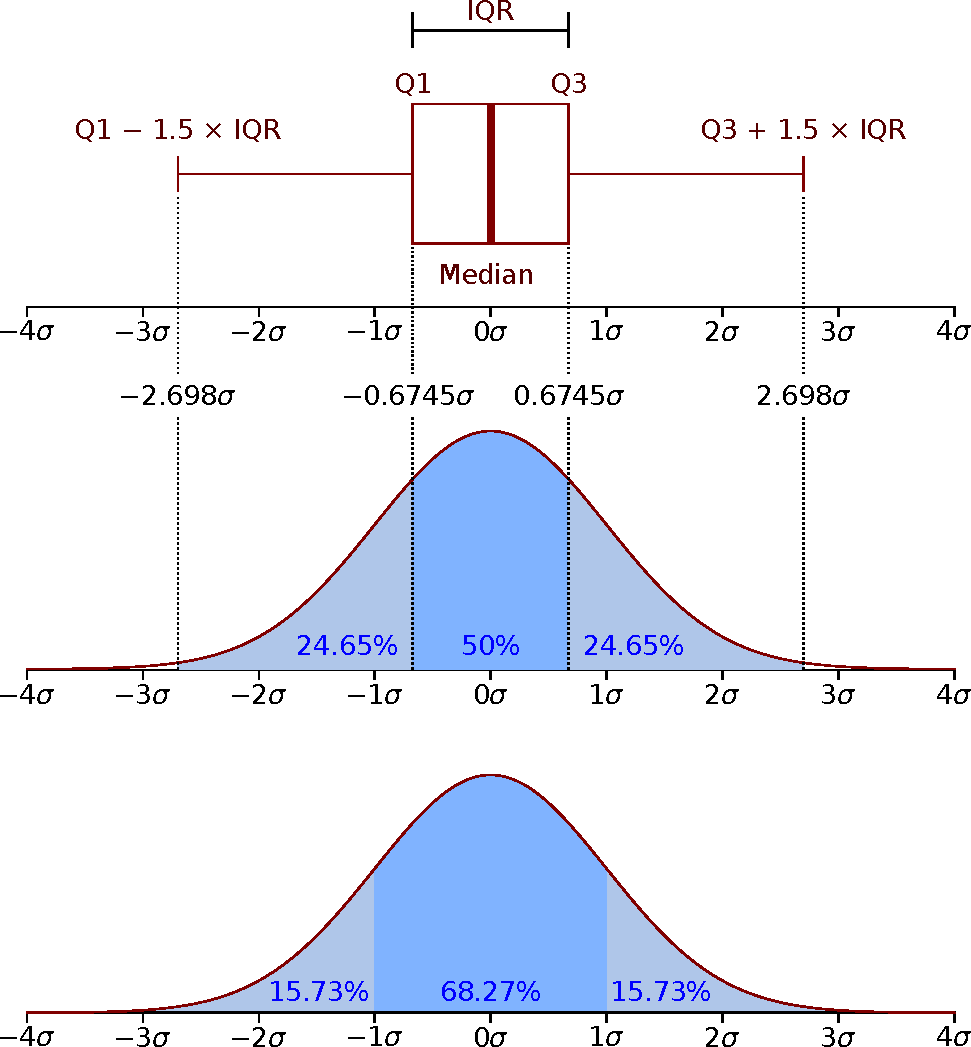
\includegraphics[width=\textwidth]{iqr_fig.pdf}
  \caption{Vemos la ubicación de los cuartiles dentro de una distribución normal, la media (\textit{Median}) también es $Q_2$.}
\end{figure}

\part{Modelos}
\section{Modelos Lineales}
Si disponemos de atributos numéricos y buscamos predecir un atributo también numérico, entonces es natural explorar los modelos lineales. Estos modelos asumen que el atributo a predecir $y^{(k)}$ responde a la forma $w_0 + \sum_i w_ix_i^{(k)}$, es decir a un hiper plano. Como se espera la presencia de errores dentro de las mediciones o simplemente se busca aproximar la forma ``real'' de $y$ se minimiza alguna métrica de distancia entre $y^{(k)}$ y $y^{(k)'} = w_o + \sum_i w_ix_i$ como pueden ser según \cite{ruppert1980trimmed}:

\begin{itemize}
\item Mínima Suma de Cuadrados
  \[
  \text{min }\sum_i (y^{(i)}-y^{(i)'})^2
  \]
\item Mínimos Valores Absolutos
  \[
  \text{min }\sum_i |y^{(i)}-y^{(i)'}|
  \]
\item M, L y S Estimadores
\item Mínima Suma Podada de Cuadrados (Least Trimmed Squares)
  \[
  \text{min }\sum_j (y^{(j)}-y^{(j)'})^2, \quad \text{donde} \quad \{ y^{(j)}-y^{(j)'} \} \subset \{ y^{(i)}-y^{(i)'} \}
  \]
\item Mínima Media de Cuadrados
  \[
  \text{min }\text{med}_i (y^{(i)}-y^{(i)'})^2
  \]
\end{itemize}

La mayor característica de los métodos lineales es, precisamente, su linealidad. Considerando que es raro encontrar un fenómeno que se comporte linealmente, la linealidad es una desventaja. Sin embargo, esto también permite que el modelo presente un menor sesgo y se verá mas adelante que esto se suele aprovechar (ver pagina \pageref{m5p}). 

Según \cite{witten2011data}, tenemos que \lstinline{LinearRegression()} utiliza la minimización de la suma de los cuadrados sin embargo dispone de un método de selección de atributos basado en el Criterio de Información de Akaike (ver página \pageref{modelselection_aic}) que simplifica el modelo resultante y está activado por defecto.
%TODO Fix reference
%TODO Add coefficients interpretation

\subsection{Ejemplos}

% TODO Check if dataset.setClassIndex es necesario
\begin{lstlisting}
  // Cargamos los datos de alguna manera
  Instances dataset = ...
  // Preparamos una instancia de prueba
  Instance testInstance = ...
  
  // Creamos una instancia del modelo
  Classifier model = new SimpleLinearRegression();
  // Entrenamos con los datos de 'dataset'
  model.buildClassifier(dataset);
  
  // Podemos imprimir los detalles del modelo
  System.out.println(model);
  // Tambien podemos predecir una instancia
  double prediction = model.classifyInstance(testInstance);
\end{lstlisting}

% TODO Check Logistic()
También podemos utilizar \lstinline{LinearRegression()}, \lstinline{MultilayerPerceptron()}\footnote{Si activamos la opción \textit{-G} (GUI) podremos modificar la topología de la red.} y con algunas modificaciones \lstinline{Logistic()}.

% Ventajas
%  bajo sesgo ?
%  simples de interpretar y de entrenar
% Desventajas
%  linealidad

\section{Árboles}
Una de las maneras usuales de atacar problemas es mediante la estrategia ``divide y conquistarás'', los arboles, con su estructura recursiva, representan fielmente esta idea. Existen multitud de variedades de árboles utilizados en minería de datos, sin embargo la idea predominante es dividir el conjunto de muestras en dos o mas subconjuntos utilizando un criterio de decisión, usualmente el valor de un atributo, y repetir esto hasta que se alcance la máxima complejidad aceptable o repetir hasta que se alcanza una predicción lo suficientemente buena.

En el caso de atributos nominales, la división es trivial y única. Para los atributos numéricos, se dispone de multitud de métodos listados en \cite{kotsiantis2006discretization} y \cite{dougherty1995supervised}. En WEKA disponemos de \lstinline{weka.filters.unsupervised.attribute.NumericToNominal} que simplemente crea una biyección entre cada valor numérico y una clase, \lstinline{weka.filters.unsupervised.attribute.Discretize} divide el atributo en clases con la misma anchura (equal-width binning) con opciones de optimización o en clases con una misma frecuencia (equal-frecuency binning) y finalmente \lstinline{weka.filters.supervised.attribute.Discretize} el cual utiliza el método MDL de Fayyad e Irani, ver \cite{irani1993multi}, que es el método por defecto utilizado en los modelos.

\subsection{\texorpdfstring{\lstinline{J48()}}{J48()}}
El modelo \lstinline{weka.classifiers.trees.J48} es el mas conocido entre los árboles presentes en WEKA, este modelo es la versión libre del algoritmo C4.5. En este modelo se construye un árbol de forma voraz seleccionando el atributo que ``mejor'' divide a las muestras. El criterio de selección está basado en la ganancia de información midiendo la diferencia de entropía entre el conjunto de datos original y el mismo conjunto de datos divido por el atributo. Intuitivamente busca maximizar la ``pureza'' de los nodos resultantes.

\[
\text{Entropía} = H = \sum_i -p_i \log_2(p_i)
\]

Veamos este ejemplo. Las muestras están clasificadas en $(0, 0, 0, 0, 1, 1, 1)$ y luego de la división según un atributo $A$ se llega $\text{right}=(0, 0, 0, 1)$ y $\text{left}=(0, 1, 1)$. Medimos la entropía de las muestras antes de la división.

\[
H_0 = -\frac{4}{7} \log\frac{4}{7} -\frac{3}{7} \log\frac{3}{7} \approx 0.985
\]
Medimos la entropía en cada subconjunto.
\[
H_{right} = -\frac{3}{4} \log\frac{3}{4} - \frac{1}{4} \log\frac{1}{4} \approx 0.811
\]
\[
H_{left} = -\frac{1}{3} \log\frac{1}{3} - \frac{2}{3} \log\frac{2}{3} \approx 0.918
\]
Obtenemos la entropía al final de la división haciendo una suma ponderada según el tamaño relativo de los subconjuntos.
\[
H_1 = \frac{4}{7}H_{right} + \frac{3}{7}H_{left} = \frac{6}{7} \approx 0.857
\]
Finalmente la Ganancia de Información, en inglés Information Gain, es la diferencia de entropías.
\[
IG = H_0 - H_1 \approx 0.128
\]

Luego de calcular la IG para cada atributo, se selecciona el mayor valor. Y se aplica recursivamente sobre los hijos. El \lstinline{J48()} aplica otros procedimientos para simplificar aún mas el árbol resultante.

\subsection{\texorpdfstring{\lstinline{RandomTree()}}{RandomTree()} y \texorpdfstring{\lstinline{RandomForest()}}{RandomForest()}} %TODO Extend
El \lstinline{Randomtree()} utiliza una estrategia simple, seleccionar aleatoriamente $k$ atributos y modela un árbol utilizándolos, finalmente no hay poda.

El modelo \lstinline{RandomForest()} construye un conjunto de \lstinline{RandomTree()}.

% TODO Extend

\subsection{Model Tree} \label{m5p}
Con \lstinline{weka.classifiers.trees.M5P} podemos construir un árbol donde sus hojas son Modelos Lineales. Es la implementación del Algoritmo M5 de J. R. Quinlan presentado en \cite{quinlan1992learning}, y utiliza la capacidad de ``simplificar'' de los árboles para terminar utilizando regresión.

% TODO EXtend

\section{Clustering}
Cuando disponemos de datos sin clasificación, tenemos un problema de clustering. En clustering se busca construir una forma de clasificar los datos según su ``similitud''. En la práctica la ``similitud'' entre dos muestras se mide con alguna métrica \cite{xu2005survey} como:
\begin{itemize}
\item Distancia de Minkowski. Para $n=1$ se reduce a D. de Manhattan, para $n=2$ se reduce a la Euclidiana.
\[
D(x, y) = \left(\sum_{i=1}^d \left(x_i-y_i\right)^{1/n}\right)^n
\]
\[
\lim_{n \to \infty} D(x, y) = \max_{1 \leq i \leq d} \left( x_i - y_i \right)
\]
\item Similitud del Coseno.
  \[
  S(i, j) = \cos \alpha = \frac{\boldsymbol{x}_i^T\boldsymbol{x}_j}{|\boldsymbol{x}_i||\boldsymbol{x}_j|}
  \]
\item Métrica ``distinto de''\cite{larose2014discovering}.
  \[
  \text{distinto}(x, y) =
  \begin{cases}
    0 & \text{Si } x = y \\
    1 & \text{Sino}
  \end{cases}
  \]
\end{itemize}

El problema de clustering es NP-difícil\cite{aloise2009np}, por ello se vuelve fácilmente computacional mente impráctico encontrar el óptimo global determinísticamente. Se suele utilizar heurísticas y distintas ejecuciones para evitar óptimos locales.
Para evitar una influencia excesiva de algún atributo se suele realizar transformaciones sobre los atributos, como Min-Max o Z-score.

\subsection{\texorpdfstring{$k$}{k}-means}
El algoritmo de $k$-means es el algoritmo de clustering mas conocido y se han propuesto múltiples modificaciones para mejorar su desempeño. % TODO Add cites
En $k$-means se inicia creando en ubicaciones aleatorias $k$ puntos los cuales serán los representantes de cada clase. Luego se itera, separando las muestras en grupos tales que una muestra pertenece a la clase representada por el punto representante mas cercano y al finalizar esto se reubican los puntos representantes en el centroide de las muestras de su clase. El algoritmo converge cuando no ocurren variaciones en las asignaciones, mide la similitud con la distancia euclidiana y busca el óptimo minimizando la suma de los cuadrados de las distancias entre las muestras y su respectivo centroide. Es muy sensible a las condiciones iniciales, es decir a las posiciones iniciales de los centroides, por ello se suele correr varias veces. La elección de la $k$ es arbitraria, puede considerarse como un parámetro mas del algoritmo y probar distintos valores o puede ser proveído por el problema, como puede ser la opinión de un experto.

Esencialmente, $k$-means es un algoritmo de optimización donde se le han definido conceptos del problema de clustering. Por ello, clustering puede ser atacado con todos los recursos ya existentes enfocados a problemas de optimización.

Una de las mejoras es $k$-means++, el cual modifica el procedimiento de inicialización de los centroides. Provee una mayor carga en la inicialización, sin embargo el tiempo total se reduce y reduce considerablemente los errores finales. Sea $D(x)$ la distancia entre la muestra $x$ y el punto representante mas cercano, entonces el algoritmo $k$-means++ es el siguiente:
\begin{enumerate}
\item Seleccionar como el primer punto representante una de las $n$ muestras con una probabilidad uniforme. Es decir, cada muestra tiene la misma probabilidad de ser seleccionada.
\item De las $n-1$ muestras, seleccionar el siguiente punto representante con una probabilidad igual a $\frac{D(x_i)^2}{\sum_j D(x_j)^2}$. Así se busca penalizar la selección de puntos cercanos a puntos representantes ya seleccionados.
\item Se repite el paso anterior hasta tener $k$ puntos representantes.
\item Continuamos con el algoritmo usual $k$-means, utilizando los puntos anteriormente seleccionados.
\end{enumerate}
Notamos que los centroides inicialmente están en las mismas posiciones que algunas muestras. Los fundamentos teóricos y datos experimentales en \cite{arthur2007k}. Existe una mejora en paralelo sobre $k$-means++ llamado $k$-means\textbar\textbar  o Scalable $k$-means++, que ofrece las mismas mejoras que $k$-means pero reduce el costo de inicialización de los centroides \cite{bahmani2012scalable}.

En WEKA usamos \lstinline{weka.clusterers.SimpleKMeans}. Con el parámetro \textit{init} controlamos el método de inicialización, con 0 la inicialización es aleatoria y con 1 la inicialización es según $k$-means++ (Existen otros métodos que soporta).

\subsection{Fuzzy Clustering}
Otra variación es la función de pertenencia de una instancia a un grupo. El algoritmo mas conocido es Fuzzy C-means, el cual es muy similar al K-means\cite{bezdek1984fcm}. Los puntos mas interesantes son:
\begin{description}
\item[La función de pertenencia] Un punto $x$ pertenece a un grupo $k$ según la función $w_k(x) \in [0, 1]$, donde $w_k(x) = 0$ sería el equivalente a no pertenecer al grupo en $k$-means y $w_k(x) = 1$ sería el equivalente a pertenecer al grupo en $k$-means.
\item[La inicialización] Los valores iniciales de $w_k(x)\quad \forall x$ son inicializados aleatoriamente
\item[La ubicación de los centroides] Los centroides son la media de todos los puntos ponderados según su pertenencia a dicho grupo.
  \[
  c_k = \frac{\sum_x w_k^m(x)x}{\sum_x w_k^m(x)}
  \]
  donde $m \geq 1$ es el ``difusificador'' (fuzzifier). $m=1$ hace que $w_k(x)$ convergen a 0 o 1 y a mayores valores de $m$ menores valores de $w_k(x)^m$ y el grupo se vuelve mas difuso.
\end{description}

\part{Evaluación}
La evaluación de un modelo es fundamental para la minería de datos ya que permite tomar las decisiones sobre que modelos desplegar, que parámetros utilizar y que comportamiento esperar.

Tanto para entrenar como para evaluar un modelo se necesitan de datos, cuando más datos se utilizan en el entrenamiento mayor aprendizaje y cuando más datos se usen en la evaluación menor varianza en la predicción, y es usual no disponer de una cantidad adecuada de datos\footnote{Los datos pueden necesitar ser obtenidos manualmente.} por ello se buscan formas de maximizar el provecho.

Un punto realmente importante es evitar que mismos datos se utilicen en ambos procedimientos. Por ejemplo, si utilizamos todos los datos para entrenar un modelo y lo evaluamos con \textbf{los mismos} datos, entonces la predicción será exageradamente optimista en algunos casos. 

\section{Holdout}
Esta estrategia de evaluación exige la existencia de 3 conjuntos de datos representativos. El conjunto de entrenamiento, \textit{training set}, el cual es utilizado para alimentar a los modelos y representa aproximadamente el 50\% de los datos originales. El conjunto de validación, \textit{validation set}, el cual es utilizado para optimizar los parámetros del modelo y se construye con un 25\%. El conjunto de pruebas, \textit{test set}, el cual es utilizado para la \textbf{evaluación final} con los 25\% finales.

Primeramente se entrena el modelo con el training set y luego se evalúa su desempeño con el validation set. Esto se repite hasta encontrar el conjunto de parámetros óptimo. Finalmente se utiliza el test set para obtener una predicción del desempeño del modelo en el despliegue. Es posible utilizar la unión de los conjuntos de entrenamiento y de validación para construir el modelo final con los parámetros optimizados y evaluarlo con el conjunto de pruebas, de esta forma se maximiza la cantidad de datos utilizado para entrenar el modelo.

Si no se dispone de 3 conjuntos de datos se puede realizar un muestreo aleatorio (o un muestreo aleatorio estratificado\footnote{Un muestreo estratificado es cuando se busca mantener la proporción de muestras según su clase.} en el caso de clase nominal) sobre el conjunto de datos.

El principal inconveniente de este método es que no se utilizan todos los datos disponibles para el entrenamiento del modelo.

\section{Cross Validation}
El ``$k$ folds Cross Validation''  se centra en utilizar toda la información disponible en los datos a costa de tiempo de computo. Primeramente se divide el conjunto de datos en $k$ subconjuntos o \textit{folds} del mismo tamaño. Luego se entrena y evalúa el modelo $k$ utilizando en cada iteración un \textit{fold} distinto para la evaluación y los demás para el entrenamiento. Luego se utiliza todo el conjunto de datos para entrenar el modelo final. Los $k$ desempeños disponibles se promedian, o se combinan de alguna manera, para obtener el desempeño del modelo final.

Así se utilizan todos los datos tanto para entrenar como para evaluar sin embargo no sobre el mismo modelo. Es evidente que la principal desventaja es la cantidad de entrenamientos y evaluaciones a realizar y además no disponemos de un procedimiento para optimizar los parámetros.

\section{Leave-one-out Cross Validation y Bootstrap}
``LoU CV'' es simplemente ``$n$ folds Cross Validation''. Esto implica un alto costo computacional mente hablando además la evaluación se realiza sobre una sola instancia lo cual garantiza un conjunto de pruebas no representativo.

``Bootstrap'' o ``0.632 Bootstrap'' hace uso del muestreo con reemplazo. Obtiene $n$ muestras con reemplazo desde el conjunto de datos de $n$ instancias y muy probablemente seleccionaremos una misma instancia varias veces podemos utilizar las instancias no seleccionadas para construir un conjunto de pruebas.

%TODO add atribute bagging

\part{Selección de Modelos}
\section{Principio de Parsimonia}
También llamado Navaja de Ockham o, en inglés, Ockham's Razor. Es un principio según el cual ``entre varias explicaciones equivalentes, se prefiere la mas simple''. 

Cabe destacar que fueron muchas las críticas contra este principio por ``ser imprudente''. La \textit{anti navaja} de A. Einstein: ``Simple, pero no más simple.''.

\section{Maximum Log-Likelihood}

\begin{figure}
  \centering
  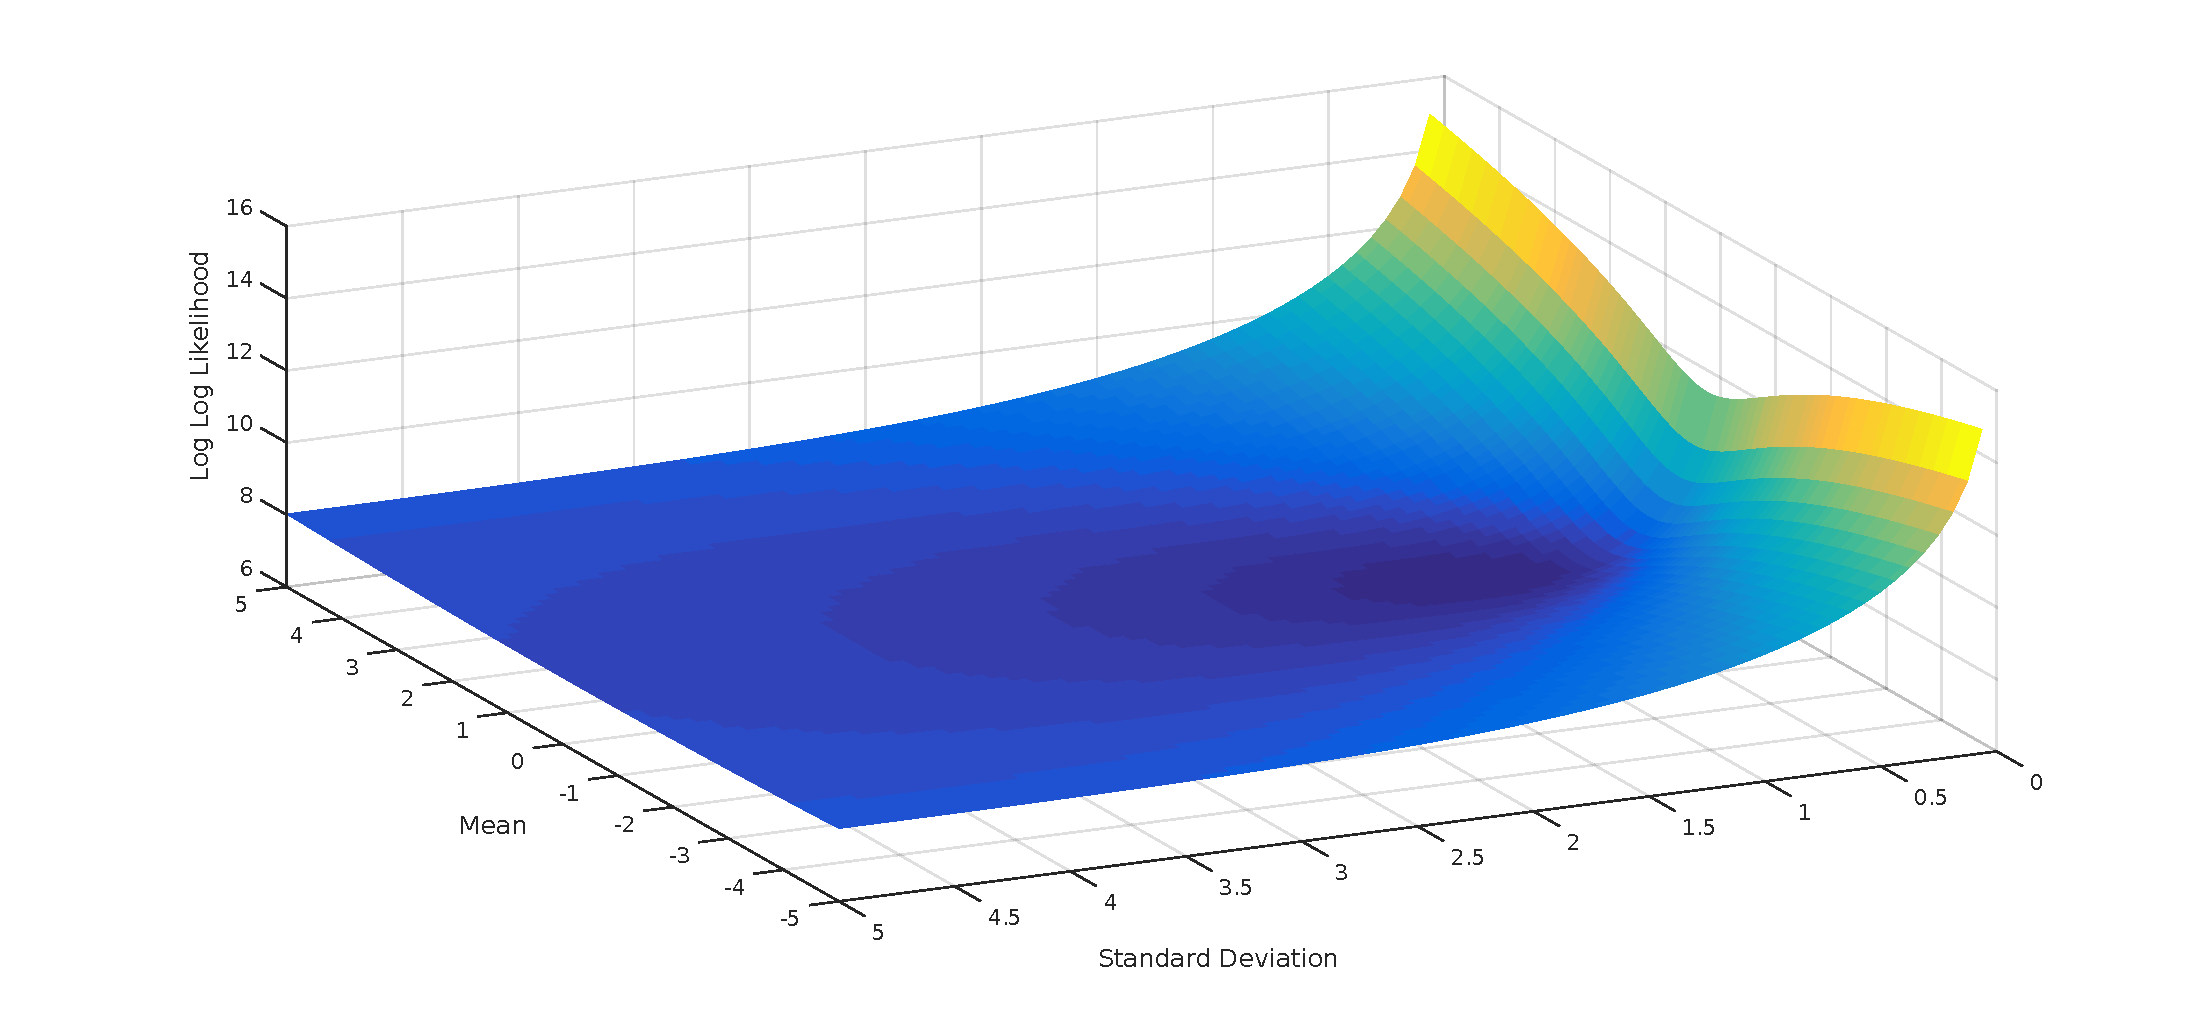
\includegraphics[width=\textwidth]{llh/normal.pdf}
  \caption{Superficie del negativo del Log-Likelihood de una Distribución Normal sobre un conjunto de datos aleatorios obtenidos a partir de $\mathcal{N}(0, 1)$.}
  \label{fig:llhplot}
\end{figure}
En español, maximización de verosimilitud. Dado un modelo con parámetros $\theta$ y un conjunto de muestras $X$ independientes e idénticamente distribuidos, la verosimilitud de los parámetros dado el conjunto de muestras $\mathcal{L}(\theta|X)$ es igual a la probabilidad de obtener las muestras dado los parámetros $P(X|\theta)$. Es decir, cual es la ``probabilidad'' de que los parámetros $\theta$ ``expliquen'' las muestras $X$.

Luego si maximizamos $\mathcal{L}(\theta|X)$ tendremos un conjunto de parámetros $\hat{\theta}$ tal que sean, o lo suficientemente cercanos a, los parámetros ``reales''\footnote{Suponiendo que el modelo ``real'' sea el mismo que el utilizado.}. Entonces tendremos que $\mathcal{L}(\theta|X) = P(X|\theta) = \prod_i P(x_i|\theta)$, sin embargo maximizar esto en la práctica es difícil por ello se busca maximizar el logaritmo de el, $\max_\theta \mathcal{L}(\theta|X) = \max_\theta \log \mathcal{L}(\theta|X) = \log \mathcal{L}(\hat{\theta}|X)= \sum_i P(x_i|\theta)$.

En la figura~\ref{fig:llhplot} de la página~\pageref{fig:llhplot}, podemos observar el negativo de una superficie de verosimilitud donde cada punto corresponde a la verosimilitud de una Distribución Normal con con media $\mu$ y desviación estándar $\sigma$ respecto a un conjunto de puntos aleatorios obtenidos desde $\mathcal{N}(0, 1)$. Como es el negativo el problema es de minimización y podemos ver como la superficie toma un mínimo para valores cercanos a $\mu=0$ y $\sigma=1$. En el código~\ref{lst:llhplot} de la página~\pageref{lst:llhplot}, disponemos de los comandos de MATLAB utilizados para generar la superficie.

En WEKA podemos utilizar \lstinline{weka.clusterers.MakeDensityBasedClusterer} para envolver cualquier algoritmo de clustering y así obtener su valor de verosimilitud.
%TODO Add code! double loglh = ClusterEvaluation.crossvalidatemodel...

\lstinputlisting[language=matlab, label={lst:llhplot}, caption={Código para generar la figura~\ref{fig:llhplot}.}]{llh/llh.m}

\section{Akaike Information Criterion}\label{modelselection_aic}
El AIC se define como $AIC = 2K - 2\ln{\mathcal{L}(\hat{\theta}|X)}$, donde $K$ es la cantidad de parámetros que se utilizaron en el modelo mas uno y $\mathcal{L}(\hat{\theta}|X)$ es el máximo de la función de verosimilitud. Este criterio indica que el modelo es ``mejor'' si posee un \textbf{menor} valor y es un criterio de comparación entre modelos \textbf{bajo los mismos datos}, es decir que el valor en si mismo no es significativo sino si el valor es menor o no al $AIC$ de otro modelo con el cual comparamos. La interpretación es la siguiente: el término $2K$ es la penalización, por tener signo positivo y estamos buscando un menor valor, por la cantidad de parámetros que el modelo posee ya que a mayor cantidad de parámetros \textbf{mayor varianza} y mayor posibilidad de ``overfitting'', por otra parte el término $-2 \ln{\mathcal{L}(\hat{\theta}|X)}$ favorece a una mejor calificación, por el tener un signo negativo, y está relacionado a verosimilitud del modelo para esos parámetros y esas muestras y también la un \textbf{menor sesgo}\cite{Hu07}.

%TODO Add critics

\part{Importación y Exportación}
\section{Exportación}
Para exportar un modelo hacemos uso de \lstinline{weka.core.SerializationHelper()} disponible desde la versión 3.5.5. Destacamos que el método \lstinline{write} también trabaja con flujos y que es necesario capturar las excepciones que arroja.
\begin{lstlisting}
  // Disponemos del modelo a exportar
  Classifier model = ...
  
  // Utilizamos el metodo .write
  String outputFilename = ...
  SerializationHelper.write(outputFilename, model);
\end{lstlisting}

\section{Importación}
Para importar utilizamos \lstinline{weka.core.SerializationHelper()} disponible desde la versión 3.5.5. Destacamos que el método \lstinline{read} también trabaja con flujos y que es necesario capturar las excepciones que arroja.
\begin{lstlisting}
  Classifier model = (Classifier) SerializationHelper.read(inputFilename);
\end{lstlisting}

\section{Trabajado en MATLAB}
Para trabajar con las herramientas que provee WEKA utilizamos \lstinline{javaaddpath} para agregar la ubicación de la biblioteca\footnote{El archivo que usualmente llamado ``weka.jar''.}.

\begin{lstlisting}{language=matlab}
  javaaddpath('weka.jar');
  import weka.classifiers.J48;
  ...
\end{lstlisting}

\printbibliography
\end{document}
